\subsubsection{13.02.15 (Competition)}
\begin{center}
	3-rd day of competition "Robofest-2015"
\end{center}
Today there were final matches.\newline

Before ad of results qualification matches we talked with all teams again and tell them about advantages that they will get if they will choose our team. So we increased our chanse to take part in a final matches if we will not get to the "top-4".\newline

When were announced results of qualification matches it turned out that our team got 4 place by the results of qualification matches. There were 3 teams in the each alliance that take part in filal matches. We refused to join to alliance of team "Pinck goose" that took 3-rd place in rating. We choose the team "Sirius"(we played very resultative match with this team) and team "Brontozabry-2007" (they could to fill 70cm of 90cm goal alone).\newline

Strategy of our alliance:
\begin{enumerate}
	\item When we play with team "Sirius" we do autonomous period from the parking zone and they ride from the ramp. In tele op period we fill the 90cm goal together. They put their balls on our gutter. In the end game they put balls into center goal and we continue filling of 90cm goal and ride to the parking zone and move 90cm goal to it.
	
	\item When we play with team "Brontozabry-2007" we do autonomous period from the parking zone and they ride from the ramp and put autonomous balls to 60cm goal. In tele op period "Brontozabry" fill 90cm goal and we fill 60cm goal. In the end game we put the balls into center goal and they move two goals and they robot to the ramp.
	
	\item When play team "Brontozabry-2007" and "Sirius" the first team do they autonomous from the ramp and "Sirius" put the balls to the center goal if the central structure is in the one position and knock the stick when it in the other two positions. In tele op they fill the 90cm goal together. Robot of the team "Brontozabry-2007" had a gutter for balls too. So "Sirius" put the balls to their gutter. In the end game "Sirius" put the balls into center goal and "Brontozabry-2007" move rolling goals to the ramp. 
\end{enumerate}


We won both rounds of the semi-final. The first round played our team and "Sirius" the second - we and "Brontozabry-2007"\newline
Actions that we did in semi-final:
\begin{enumerate}
	\item 1-st round:
	\begin{itemize}
		\item In autonomous period we put the balls into 30cm goal and 90cm goal (60 points). Team "Sirius" didn't ride from the ramp.
		
		\item In tele op period we and "Sirius" filled 90cm completely (261 point).
		
		\item In the end game "Sirius" coundn't put balls into center goal and they ride to the parking zone. We moved 90cm goal and our robot to the parking zone (30 points).
		
		\item Total: 351 point 
	\end{itemize}
		\item 2-nd round:
		\begin{itemize}
			\item In autonomous period we put the balls into 30cm goal and 90cm goal (60 points). Team "Brontozabry-2007" moved out from the ramp and put autonomous balls into 60cm goal (50 points).
			
			\item In tele op period "Brontozabry-2007" filled 70cm of 90cm goal (210 points) and we filled 30cm of 60cm goal (60 points).
			
			\item In the end game we put 3 big balls and 1 small to the center goal (about 140 points). The second team moved 60cm and 90cm goal and their robot to the ramp (90 points). Also we moved our robot to the parking zone (10 points).
			
			\item Total: 620 points
		\end{itemize}
\end{enumerate}

One team from the second alliance-finalist blocked the way to rolling goals in autonomous period. So it was decided that our team will not take a part in the match against this team. We won both round of the final match. The first round played our team and team "Brontozabry-2007". The second round played "Sirius" and "Brontozabry".\newline
Actions that we did in final:
\begin{enumerate}
	\item 1-st round:
	\begin{itemize}
		\item In autonomous period we put balls into 60cm goal and 90 cm goal and moved 90cm goal to the parking zone (80 points). The 30 cm goal we lost because it hit central structure due to low accuracy of turning. The second team moved out frome the ramp and put autonomous balls to 60cm goal (50 points).
		
		\item In tele op period we filled 60cm goal completely (114 points). "Brontozabry-2007" filled 70cm of 90cm goal (210 points).
		
		\item In the end game we put 4 big balls into center goal (162 points). The second team moved 60cm and 90cm goals and their robot to the ramp (90 points). Also we moved our robot to the parking zone (10 points).
		
		\item Total: 716 points.
	\end{itemize}
		\item 2-nd round:
		\begin{itemize}
			\item In autonomous period "Sirius" knocked the stick (30 points). "Brontozabry" moved out from the ramp(20 points). They didn't put autonomous balls to rolling goal because one opponent blocked the way to rolling goal.
			
			\item In tele op period they filled 75cm of 90cm goal (225 points).
			
			\item In the end game "Brontozabry-2007" moved 60cm and 90cm goals and their robot to the ramp (90 points). "Sirius" couldn't put 4 big balls to center goal because opponent pushed them and balls fell to floor. But they still managed capture one big and one small balls and put them to cener goal (60 points).
			
			\item Total: 425 points.
		\end{itemize}
\end{enumerate}


So our alliance won in categotry FIRST FTC.\newline

Внесенные доработки:
\begin{enumerate}
	\item The traectory of moving to the parking zone in autonomous period was changed so that our robot doesn't hit our ally that moved out from the ramp.
	\begin{figure}[H]
		\begin{minipage}[h]{0.2\linewidth}
			\center  
		\end{minipage}
		\begin{minipage}[h]{0.6\linewidth}
			\center{
\includegraphics[scale=0.8]{days/13.02.15/images/01}}
			\caption{Black line - old traectory, red line - new}
		\end{minipage}
	\end{figure}
	
\end{enumerate}

Results of competition:
\begin{enumerate}
	\item We took 4 place by the results of qualification matches.
	
	\item Our alliance won semi-final and final.
	
	\item Our team took the first place in team standings.
	
	\item We didn't tale prize places in nomination "Engineering book".
	
	\item We didn't tale prize places in other nomination.
\end{enumerate}

Summing up:
\begin{enumerate}
	\item Success in competition:
	\begin{enumerate}
		\item We took the 1-st place in team standings and got the rule to take a part in FIRST World Championship that will be in Saint-Louis, USA.
		
		\item We won 6 matches from 7 (4 qualification and 3 final matches).
		
		\item Due to trainings our operators control the robot successfuly worked competently and coordinated their actions with each other and with operators of ally.
		
		\item Mechanisms worked stability and didn't brake except partially failure of MOB (unlike the previous competition).
		
		\item Programme of autonomous period worked not very stable and we got only half from planned points  on average.
		
		\item Programme of tele op worked stabil.
		
	\end{enumerate}
	
	\item Our mistakes and disadvantages of construction:
	\begin{enumerate}
		\item Although we made intermediate position of the bucket jam of balls was a problem and we wasted time due to it.
		
		\item We couldn't move when lift rised because small balls can get under the robot and prevent to lowering bucket. If we'll make stationary ramp this problem will solved.
		
	\end{enumerate}
	
	\item Useful ideas that we took from another teams:
	\begin{enumerate}
		\item Robot of the team from Moscow "Indigo" had a mechanism that can rise rolling goal in allows to get 30 points and don't move rolling goal to the ramp.
		\begin{figure}[H]
			\begin{minipage}[h]{0.2\linewidth}
				\center  
			\end{minipage}
			\begin{minipage}[h]{0.6\linewidth}
				\center{
\includegraphics[scale=0.25]{days/13.02.15/images/02}}
				\caption{Mechanism that rises the rolling goal}
			\end{minipage}
		\end{figure}
		
		\item Robot of the Romanian team "AutoVortex Black Edition" had a wheel base that consist of 6 standard wheels that can rotates around vertical axis. It allows to robot move in all directions and prevent to problems that has robot with omni-wheels: sliping of wheels and low accuracy of moving by encoders and problem with riding to the ramp.
		\begin{figure}[H]
			\begin{minipage}[h]{0.2\linewidth}
				\center  
			\end{minipage}
			\begin{minipage}[h]{0.6\linewidth}
				\center{
\includegraphics[scale=0.2]{days/13.02.15/images/03}}
				\caption{Robot of Romanian team (wheel base is not showed)}
			\end{minipage}
		\end{figure}
		
		\item Robot of the team "Indigo" had a additional grippers that was fixed on the sides. This grippers moved balls to the main gripper. It effective when balls are near the wall and main gripper can't get them. In addition operators doesn't need to aim to the ball and if robot push ball it not away from it. 
		\begin{figure}[H]
			\begin{minipage}[h]{0.47\linewidth}
				\center{
\includegraphics[scale=0.2]{days/13.02.15/images/04}}
			\end{minipage}
			\hfill
			\begin{minipage}[h]{0.47\linewidth}
				\center{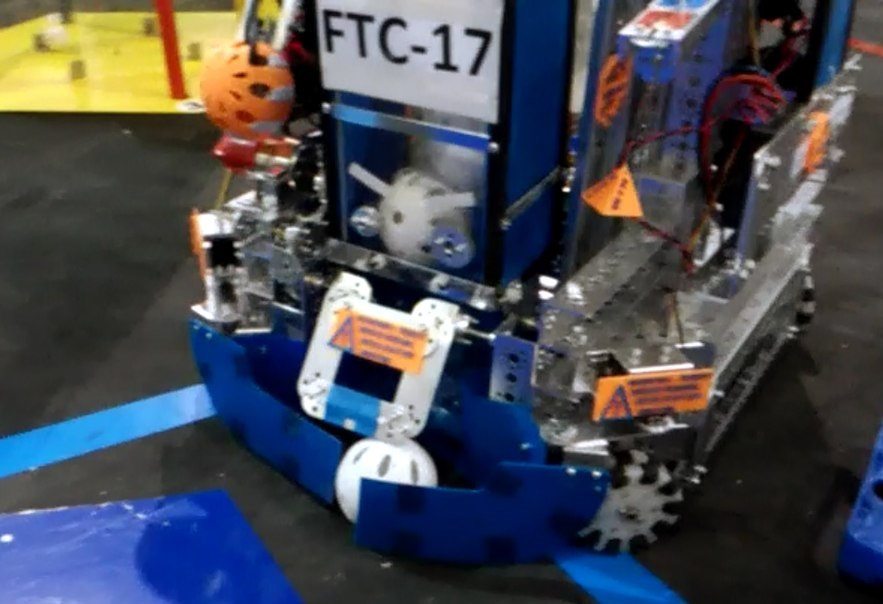
\includegraphics[scale=0.21]{days/13.02.15/images/05}}
			\end{minipage}
			\caption{Side grippers}
		\end{figure}
		
	\end{enumerate}
	
	\item Tasks for the next meeting:
	\begin{enumerate}
		\item To make the mechanism that rise the rolling goal.
		
		\item To make the autonomous period so that robot put the balls to center goal and knock the stick.
		
		\item To make turning in autonomous period by giro. It more accurate than encoders
		
		\item To make side grippers for balls.
		
		\item To make 3-d model of robot more accurate and detalied.
		
		\item To make the bucket where balls will not stuck.
			
		\item To make stationary ramp for balls.
		
		\item To increase power of MOB so that it can overturn bucket with 5 balls.
		
	\end{enumerate}
	
\end{enumerate}
\fillpage